\documentclass[11pt,a4paper]{report}
\usepackage[utf8]{inputenc}
\usepackage{amsmath}
\usepackage{graphicx}
\usepackage{tabularx}
\usepackage{adjustbox}
%\usepackage[colorinlistoftodos]{todonotes}
\usepackage{csquotes}
\usepackage{comment}
\usepackage{imakeidx}
%tabela
\usepackage{multirow}
\usepackage{xcolor}
\usepackage[margin=3cm]{geometry}
\usepackage[hidelinks]{hyperref}
\usepackage[toc,acronym,nopostdot,nonumberlist]{glossaries}
\usepackage{titling}
\usepackage{tikzpagenodes}
\usepackage[ddmmyyyy]{datetime}
\usepackage{setspace}
\usepackage{indentfirst}

%para definir a localização das tabelas e imagens em modo strict
%\usepackage{placeins}

\usepackage{biblatex}
\addbibresource{ref.bib}
\makeglossaries

%colocar aqui variáveis que serão utilizadas no texto:
\newcommand\kbps{\text{\textit{k}bit/s}}
\doublespacing

\begin{document}

\begin{titlepage}
\begin{tikzpicture}[remember picture,overlay,shift={(current page.center)}]
\node[anchor=center,xshift=-3cm,yshift=9cm]{
\includegraphics[scale=0.25]{figs/MCiber-logo.pdf}};
\node[anchor=center,xshift=3cm,yshift=8.3cm]{
\includegraphics[scale=0.65]{figs/letter-MCiber.pdf}};
\node[anchor=center,xshift=7cm,yshift=-12cm]{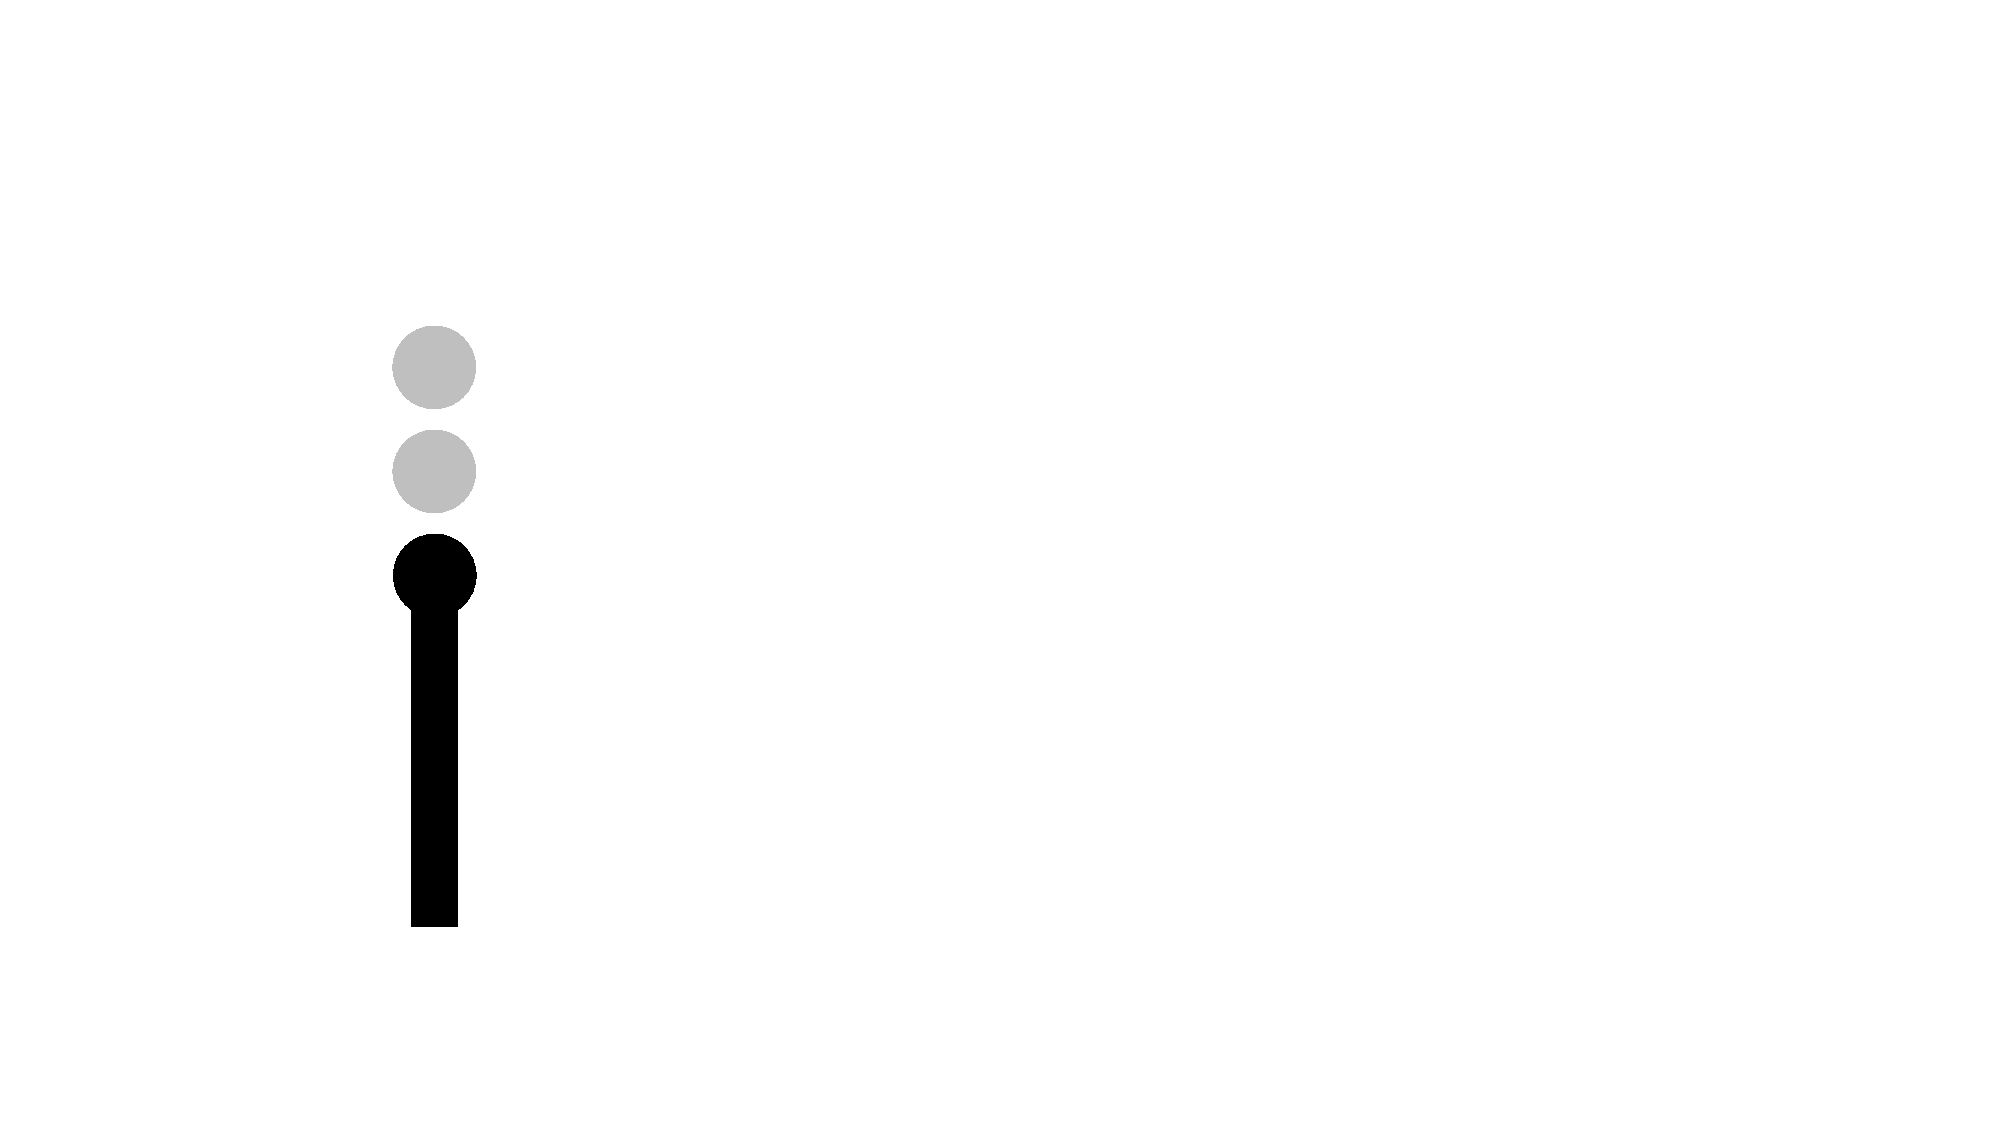
\includegraphics[scale=0.7]{figs/MCiber-end2.pdf}};
\end{tikzpicture}

\centering
\vspace{7cm}
\huge Title of the Project\\
\vspace{2cm}
\large a Thesis authored by\\
%\large a lab assignment report authored by\\
\Large Name of the student\\
\vspace{3cm}
\large supervised by\\
\large Prof. X and Prof. Y\\
\vspace{2cm}
\newdateformat{daymonthyear}{\THEDAY\ \monthname[\THEMONTH], \THEYEAR}
\daymonthyear\today \\
\vspace{1cm}

\includegraphics[scale=0.4]{figs/ESTG-logo.png}
%December, 2019
%\large v2.3
\end{titlepage}

%%%% colocar aqui acrónimos
\newacronym{mcyber}{MCyber}{Master in Cybersecurity}
\newacronym{wn}{WN}{Wireless Network}

%%%%%%%%%%%%%%%%%%%%%%%%%%%%%%%%%%%%%%%%%%%%%%%%%%%%%
\begin{abstract}
context
The quick brown fox jumps over the lazy dog. The quick brown fox jumps over the lazy dog. The quick brown fox jumps over the lazy dog. The quick brown fox jumps over the lazy dog. The quick brown fox jumps over the lazy dog. The quick brown fox jumps over the lazy dog.

\end{abstract}


\textbf{Keywords:} word1. word2. word3. word4.

%insert index
\tableofcontents
\glsaddall
\printglossary[type=\acronymtype]
\printglossary[type=main,title={Glossary},toctitle={Glossary}]
%%%%%%%%%%%%%%%%%%%%%%%%%%%%%%%%%%%%%%%%%%%%%%%%%%%%%

\chapter{Introduction}
\label{chap:introduction}

In this Chapter ...

IMPORTANT:
\begin{itemize}
    \item PLEASE check the file vars.tex: I'm using it in 10\kbps.
    \item Using glossaries for the first time: \gls{wn}
    \item Using glossaries after first time: \gls{wn}
    \item Using glossaries in plural: \glspl{wn}
    \item Using glossaries extended: \glsdesc{wn}
\end{itemize}

How to reference and insert a figure \ref{fig:labeloffigure}.

\begin{figure}[ht]
    \centering
    
\includegraphics[scale=0.2]{figs/MCiber-logo.pdf}
    \caption{This is a figure}
    \label{fig:labeloffigure}
\end{figure}

This is an example of a citation \cite{Pedro2019}.

This is a way for you to generate tables:

https://www.tablesgenerator.com/

The quick brown fox jumps over the lazy dog. The quick brown fox jumps over the lazy dog. The quick brown fox jumps over the lazy dog. The quick brown fox jumps over the lazy dog. The quick brown fox jumps over the lazy dog. The quick brown fox jumps over the lazy dog.

\section{Context}
\label{sec:context}
%Context
The quick brown fox jumps over the lazy dog. The quick brown fox jumps over the lazy dog. The quick brown fox jumps over the lazy dog. The quick brown fox jumps over the lazy dog. The quick brown fox jumps over the lazy dog. The quick brown fox jumps over the lazy dog.

%context focus
The quick brown fox jumps over the lazy dog. The quick brown fox jumps over the lazy dog. The quick brown fox jumps over the lazy dog. The quick brown fox jumps over the lazy dog. The quick brown fox jumps over the lazy dog. The quick brown fox jumps over the lazy dog.

\section{Problem Statement and Motivation}
\label{sec:motivation}
%problem to solve
The quick brown fox jumps over the lazy dog. The quick brown fox jumps over the lazy dog. The quick brown fox jumps over the lazy dog. The quick brown fox jumps over the lazy dog. The quick brown fox jumps over the lazy dog. The quick brown fox jumps over the lazy dog.

%point the motivation
The motivation of the current project is
The quick brown fox jumps over the lazy dog. The quick brown fox jumps over the lazy dog. The quick brown fox jumps over the lazy dog. The quick brown fox jumps over the lazy dog. The quick brown fox jumps over the lazy dog. The quick brown fox jumps over the lazy dog.

\section{Objectives}
\label{sec:name}
The general objective is to
The quick brown fox jumps over the lazy dog. The quick brown fox jumps over the lazy dog. The quick brown fox jumps over the lazy dog. The quick brown fox jumps over the lazy dog. The quick brown fox jumps over the lazy dog. The quick brown fox jumps over the lazy dog.

\section{Organization}
\label{sec:org}
The quick brown fox jumps over the lazy dog. The quick brown fox jumps over the lazy dog. The quick brown fox jumps over the lazy dog. The quick brown fox jumps over the lazy dog. The quick brown fox jumps over the lazy dog. The quick brown fox jumps over the lazy dog.

\chapter{Title of the chapter}
\label{cap:name1}

The quick brown fox jumps over the lazy dog. The quick brown fox jumps over the lazy dog. The quick brown fox jumps over the lazy dog. The quick brown fox jumps over the lazy dog. The quick brown fox jumps over the lazy dog. The quick brown fox jumps over the lazy dog.

\section{Section 1}
\label{sec:sec1}

The quick brown fox jumps over the lazy dog. The quick brown fox jumps over the lazy dog. The quick brown fox jumps over the lazy dog. The quick brown fox jumps over the lazy dog. The quick brown fox jumps over the lazy dog. The quick brown fox jumps over the lazy dog.

\begin{itemize}
    \item The quick brown fox jumps over the lazy dog. The quick brown fox jumps over the lazy dog. The quick brown fox jumps over the lazy dog. The quick brown fox jumps over the lazy dog. The quick brown fox jumps over the lazy dog. The quick brown fox jumps over the lazy dog.
    \item The quick brown fox jumps over the lazy dog. The quick brown fox jumps over the lazy dog. The quick brown fox jumps over the lazy dog. The quick brown fox jumps over the lazy dog. The quick brown fox jumps over the lazy dog. The quick brown fox jumps over the lazy dog.
\end{itemize}

%%%%%%%%%%%%%%%%%%%%%%%%%%%%%%%%%%%%%%%%%%%%%%%%%%%%%
\chapter{Title of the chapter}
\label{cap:name2}

The quick brown fox jumps over the lazy dog. The quick brown fox jumps over the lazy dog. The quick brown fox jumps over the lazy dog. The quick brown fox jumps over the lazy dog. The quick brown fox jumps over the lazy dog. The quick brown fox jumps over the lazy dog.

\section{Section 2}
\label{sec:sec2}

The quick brown fox jumps over the lazy dog. The quick brown fox jumps over the lazy dog. The quick brown fox jumps over the lazy dog. The quick brown fox jumps over the lazy dog. The quick brown fox jumps over the lazy dog. The quick brown fox jumps over the lazy dog.


\addcontentsline{toc}{chapter}{References}
\printbibliography[title={References}]

\end{document}
